\documentclass[11pt]{book}

%%%%%%%%%%%%%%Include Packages%%%%%%%%%%%%%%%%%%%%%%%%%%
\usepackage{xcolor}
\usepackage{mathtools}
\usepackage[legalpaper, total={6in, 8in}, margin=1.25in]{geometry}
\usepackage{amsmath}
\usepackage{amssymb}
\usepackage{paralist}
\usepackage{rsfso}
\usepackage{amsthm}
\usepackage{wasysym}
\usepackage[inline]{enumitem}   
\usepackage{hyperref}
\usepackage{tocloft}
\usepackage{wrapfig}
\usepackage{titlesec}
\usepackage{colortbl}
\usepackage{stackengine} 
\usepackage{csvsimple}
\usepackage{listings}
%%%%%%%%%%%%%%%%%%%%%%%%%%%%%%%%%%%%%%%%%%%%%%%%%%%%%%%%



%%%%%%%%%%%%%%%Code%%%%%%%%%%%%%%%%%%%%%%%%%%%%%%%%%%%%%
\definecolor{codegreen}{rgb}{0,0.6,0}
\definecolor{codegray}{rgb}{0.5,0.5,0.5}
\definecolor{codepurple}{rgb}{0.58,0,0.82}
\definecolor{backcolour}{rgb}{0.95,0.95,0.92}

\lstdefinestyle{mystyle}{
    backgroundcolor=\color{backcolour},   
    commentstyle=\color{codegreen},
    keywordstyle=\color{magenta},
    numberstyle=\tiny\color{codegray},
    stringstyle=\color{codepurple},
    basicstyle=\ttfamily\footnotesize,
    breakatwhitespace=false,         
    breaklines=true,                 
    captionpos=b,                    
    keepspaces=true,                 
    numbers=left,                    
    numbersep=5pt,                  
    showspaces=false,                
    showstringspaces=false,
    showtabs=false,                  
    tabsize=2
}
%%%%%%%%%%%%%%%%%%%%%%%%%%%%%%%%%%%%%%%%%%%%%%%%%%%%%%%%




%%%%%%%%%%%%%%%Chapter Setting%%%%%%%%%%%%%%%%%%%%%%%%%%
\definecolor{gray75}{gray}{0.75}
\newcommand{\hsp}{\hspace{20pt}}
\titleformat{\chapter}[hang]{\Huge\bfseries}{\thechapter\hsp\textcolor{gray75}{$\mid$}\hsp}{0pt}{\Huge\bfseries}
%%%%%%%%%%%%%%%%%%%%%%%%%%%%%%%%%%%%%%%%%%%%%%%%%%%%%%%%

%%%%%%%%%%%%%%%%%Theorem environments%%%%%%%%%%%%%%%%%%%
\newtheoremstyle{break}
  {\topsep}{\topsep}%
  {\itshape}{}%
  {\bfseries}{}%
  {\newline}{}%
\theoremstyle{break}
\theoremstyle{break}
\newtheorem{axiom}{Axiom}
\newtheorem{thm}{Theorem}[section]
\renewcommand{\thethm}{\arabic{section}.\arabic{thm}}
\newtheorem{lem}{Lemma}[thm]
\newtheorem{prop}[lem]{Proposition}
\newtheorem{corL}{Corollary}[lem]
\newtheorem{corT}[lem]{Corollary}
\newtheorem{defn}{Definition}[corL]
\newenvironment{indEnv}[1][Proof]
  {\proof[#1]\leftskip=1cm\rightskip=1cm}
  {\endproof}
%%%%%%%%%%%%%%%%%%%%%%%%%%%%%%%%%%%%%%%%%%%%%%%%%%%%%%


%%%%%%%%%%%%%%%%%%%%%%%Integral%%%%%%%%%%%%%%%%%%%%%%%
\def\upint{\mathchoice%
    {\mkern13mu\overline{\vphantom{\intop}\mkern7mu}\mkern-20mu}%
    {\mkern7mu\overline{\vphantom{\intop}\mkern7mu}\mkern-14mu}%
    {\mkern7mu\overline{\vphantom{\intop}\mkern7mu}\mkern-14mu}%
    {\mkern7mu\overline{\vphantom{\intop}\mkern7mu}\mkern-14mu}%
  \int}
\def\lowint{\mkern3mu\underline{\vphantom{\intop}\mkern7mu}\mkern-10mu\int}
%%%%%%%%%%%%%%%%%%%%%%%%%%%%%%%%%%%%%%%%%%%%%%%%%%%%%%



\newcommand{\R}{\mathbb{R}}
\newcommand{\N}{\mathbb{N}}
\newcommand{\Z}{\mathbb{Z}}
\newcommand{\Q}{\mathbb{Q}}
\newcommand{\C}{\mathbb{C}}
\newcommand{\T}{\mathcal{T}}
\newcommand{\M}{\mathcal{M}}
\newcommand{\Symm}{\text{Symm}}
\newcommand{\Alt}{\text{Alt}}
\newcommand{\Int}{\text{Int}}
\newcommand{\Bd}{\text{Bd}}
\newcommand{\Power}{\mathcal{P}}
\newcommand{\ee}[1]{\cdot 10^{#1}}
\newcommand{\spa}{\text{span}}
\newcommand{\sgn}{\text{sgn}}
\newcommand{\degr}{\text{deg}}
\newcommand{\pd}{\partial}
\newcommand{\that}[1]{\widetilde{#1}}
\newcommand{\lr}[1]{\left(#1\right)}
\newcommand{\vmat}[1]{\begin{vmatrix} #1 \end{vmatrix}}
\newcommand{\bmat}[1]{\begin{bmatrix} #1 \end{bmatrix}}
\newcommand{\pmat}[1]{\begin{pmatrix} #1 \end{pmatrix}}
\newcommand{\rref}{\xrightarrow{\text{row\ reduce}}}
\newcommand{\txtarrow}[1]{\xrightarrow{\text{#1}}}
\newcommand\oast{\stackMath\mathbin{\stackinset{c}{0ex}{c}{0ex}{\ast}{\Circle}}}


\newcommand{\note}{\color{red}Note: \color{black}}
\newcommand{\remark}{\color{blue}Remark: \color{black}}
\newcommand{\example}{\color{green}Example: \color{black}}
\newcommand{\exercise}{\color{green}Exercise: \color{black}}

%%%%%%%%%%%%%%%%%%%%%%Roman Number%%%%%%%%%%%%%%%%%%%%%%%
\makeatletter
\newcommand*{\rom}[1]{\expandafter\@slowromancap\romannumeral #1@}
\makeatother
%%%%%%%%%%%%%%%%%%%%%%%%%%%%%%%%%%%%%%%%%%%%%%%%%%%%%%%%%

%%%%%%%%%%%%table of contents%%%%%%%%%%%%%%%%%%%%%%%%%%%%
\setlength{\cftchapindent}{0em}
\cftsetindents{section}{2em}{3em}

\renewcommand\cfttoctitlefont{\hfill\huge\bfseries}
\renewcommand\cftaftertoctitle{\hfill\mbox{}}

\setcounter{tocdepth}{2}
%%%%%%%%%%%%%%%%%%%%%%%%%%%%%%%%%%%%%%%%%%%%%%%%%%%%%%%%%


%%%%%%%%%%%%%%%%%%%%%Footnotes%%%%%%%%%%%%%%%%%%%%%%%%%%%
\newcommand\blfootnote[1]{%
  \begingroup
  \renewcommand\thefootnote{}\footnote{#1}%
  \addtocounter{footnote}{-1}%
  \endgroup
}
%%%%%%%%%%%%%%%%%%%%%%%%%%%%%%%%%%%%%%%%%%%%%%%%%%%%%%%%%

%%%%%%%%%%%%%%%%%%%%%Section%%%%%%%%%%%%%%%%%%%%%%%%%%%%%
\makeatletter
\def\@seccntformat#1{%
  \expandafter\ifx\csname c@#1\endcsname\c@section\else
  \csname the#1\endcsname\quad
  \fi}
\makeatother
%%%%%%%%%%%%%%%%%%%%%%%%%%%%%%%%%%%%%%%%%%%%%%%%%%%%%%%%%

%%%%%%%%%%%%%%%%%%%%%%%%%%%%%%%%%%%Enumerate%%%%%%%%%%%%%%
\makeatletter
% This command ignores the optional argument 
% for itemize and enumerate lists
\newcommand{\inlineitem}[1][]{%
\ifnum\enit@type=\tw@
    {\descriptionlabel{#1}}
  \hspace{\labelsep}%
\else
  \ifnum\enit@type=\z@
       \refstepcounter{\@listctr}\fi
    \quad\@itemlabel\hspace{\labelsep}%
\fi}
\makeatother
\parindent=0pt
%%%%%%%%%%%%%%%%%%%%%%%%%%%%%%%%%%%%%%%%%%%%%%%%%%%%%%%%%%


\begin{document}

	\begin{titlepage}
		\begin{center}
			\vspace*{1cm}
			\Huge \color{red}
				\textbf{Lab 3 Report}\\
			\vspace{0.5cm}			
			\Large \color{black}
				Math 391 - Introduction to Modern Physics Lab\\
				Professor Wayne Lau\\	
				University of Michigan\\
			\vspace{3cm}

			
\includegraphics[scale=0.8]{Jinyan'sQuestion.pdf}
			
			
			\vspace{5cm}
			\LARGE
				\textbf{Jinyan Miao}\\
				\hfill\break
				\LARGE Fall 2022\\
			\vspace{1cm}

		\vspace*{\fill}
		\end{center}			
	\end{titlepage}


\newpage
\tableofcontents
\addtocontents{toc}{~\hfill\textbf{Page}\par}


\setcounter{chapter}{3}
\chapter*{Lab 3 - Photoelectric Effect}
\section{Introduction}
In 1887, Heinrich Hertz discovered that light would cause the ejection of electrons from the surface of metals, so-called the photoelectric effect.$^{[1]}$ Einstein, aware of Planck's theory on photon energy quantization, theorized that the photoelectric effect was a result of the electrons absorbing individual quanta of light, or a photon, with energy proportional to the frequency, and he proposed that the universal relationship between the maximal energy $E_{max}$ of the ejected electron and the frequency $f$ of the incident light is given by the following:$^{[2]}$
\begin{align}
E_{max} = hf - e\phi
\end{align}
where $f$ is Planck's constant and $e\phi$ is the work function for the photoelectron-emitting surface. Here we note that (3.1) is valid only when we have $hf\geq e\phi$. \\

Phototube is a type of light sensor that operates according to equation (3.1). When incoming photons strike the photocathode, electrons are knocked out of the surface of the cathode. The electrons are then attracted to an anode hence causing a current. If one applies variable retarding potential across the phototube, then by (3.1), one can find a stopping voltage $V_s$ such that there is no current presented in the phototube, in which case we can write:
\begin{align}
eV_s =E_{max}= hf - e\phi
\end{align}
In Lab 3 of Physics 391, we verified that, as suggested by (3.2), the stopping voltage $V_s$ is independent of the intensity of the incident light but dependent on the frequency of the incident light. We used the Hamamatsu R414 phototube in our experiment, whose cathode material is cesium antimonide. We found that for incident light is of wavelength $405\, nm$, $532\, nm$, and $635\, nm$, the stopping voltage is given by $1.339\pm 0.038\, V$, $0.671\pm 0.009\, V$, and $0.391\pm 0.007\, V$, respectively. We also estimated the Planck's constant using equation (3.2) with our data, and the estimated Planck's constant is $(5.8776\pm 0.2838) \cdot 10^{-34}\, m^2 \, kg/s$. 

\hfill\break
\hfill\break
\section{Experimental setup}
In this experiment, we use the Hamamatsu R414 phototube. The phototube is placed in a photoelectric effect apparatus (a box-shape equipment), and is wired to a source such that retarding voltage can be applied across the phototube. A laser pointer is then slipped in to the apparatus. When the laser is turned on, it serves as a photon source causing the electron on the cathode of the phototube to be ejected. The values for photocurrents in our setup is too low for detection with normal instruments, so instead we measure the voltage across an $10000\,\Omega$ resistor connecting the anode to ground, and that voltage of the resistor is directly proportional to the current in the phototube. As we vary the retarding voltage across the phototube, both the retarding voltage and the corresponding voltage across anode resistor are recorded. We repeat this procedure for three laser pointers emitting light in three different wavelengths, $405\, nm$, $532\, nm$, and $635\, nm$. We then repeat the experiment with an optical neutral density filter slipped across the laser tube. The density filter has transmitted fraction $10^{-0.3}$. Six sets of data are collected in total, three for lasers without the filter, and three for lasers with the filter.
\\
 
\newpage
\section{Visualizing the data}
The recorded voltage across the anode with corresponding voltage across the cathode is displaced in the following plots for the three lasers:\\
\begin{center}
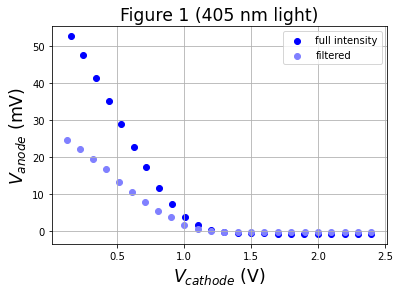
\includegraphics[scale=0.5]{fig1.png}\qquad
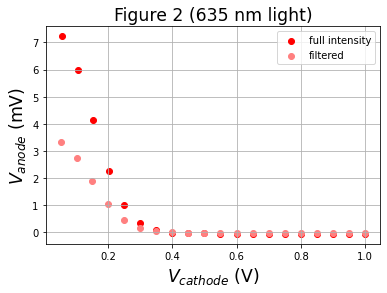
\includegraphics[scale=0.5]{fig2.png}\\
\hfill\break
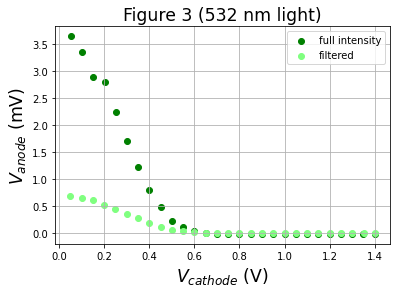
\includegraphics[scale=0.45]{fig3.png}
\end{center}
We notice the small shift between the third and the forth dark green data points on the upper left in Figure 3. The multimeter recording the cathode voltage stopped working while we performed the measurement, and we swithced to a new one. The shift in the data points is most likely due to the slight calibration difference of the multimeter. When analyzing the data for the $532\, nm$ laser, for consistency, we neglect the first three data points. 

\hfill\break
\hfill\break
\hfill\break
\section{Analyzing the data}
\subsection{Determining the stopping voltage}
In order to find the stopping voltage $V_s$ for each case, we fit our data points to the following function, which gives a good mathematical model for the photocurrent according to the Lab Manual:
\begin{align}
i_{photo} = \frac{a(V_s - V)^2\theta(V_s - V) + b(V_S - V)^4 \theta(V_s -V)}{1+c(V_s - V)^2 \theta(V_S-V)}
\end{align}
where $i_{photo}$ is the photocurrent directly proportional to $V_{anode}$, $V$ is $V_{cathode}$, and $\theta$ is the unit step function defined by the following:
\begin{align*}
\theta: \R \to \{0,1\} \qquad x\mapsto \begin{cases}
0 & x<0 \\
1 & x\geq 0
\end{cases}
\end{align*}
Note that the ratio $V_{anode}/i_{photo}$ is resolved in the parameters $a$ and $b$ in (3.3), hence we can fit (3.3) by replacing $i_{photo}$ as $V_{anode}$ without affecting the best fit value for $V_s$. We fit the data points using the Python scipy function \textit{optimize.curve$\_$fit}.\\
\newpage
First, we perform the fitting procedure for the reduced-intensity light data. For the incident light of wavelength $635\, nm$, the best fit values and the standard deviations of the parameters are given by the followings:
\begin{center}
\begin{tabular}{|c|c|c|c|c|}
\hline
 & a & b & c & $V_s$\\
\hline
best fit value & 257.1805 & -899.2726 & -12.2266 & 0.3887\\
\hline
standard deviation & 21.2474 & 97.0962 & 3.7728 & 0.0069 \\
\hline
\end{tabular}\\
\hfill\break
\hfill\break
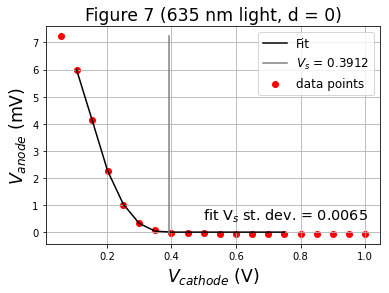
\includegraphics[scale=0.5]{fig7.png}
\end{center}
Here the stopping voltage for reduced-intensity light of $\lambda = 635\, nm$ is $0.3887\pm 0.0069\, V$. \\

For the reduced-intensity light of wavelength $532\, nm$, the fitted parameters are given by:
\begin{center}
\hfill\break
\begin{tabular}{|c|c|c|c|c|}
\hline
 & a & b & c & $V_s$\\
\hline
best fit value & 14.3785 & -20.6220 & -0.0516 & 0.6786\\
\hline
standard deviation & 2.6529 & 4.9268 & 3.5398 & 0.0139 \\
\hline
\end{tabular}\\
\hfill\break
\hfill\break
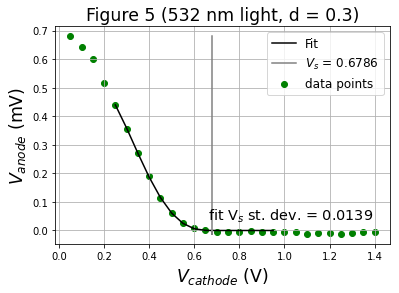
\includegraphics[scale=0.5]{fig5.png}
\end{center}
Here the stopping voltage for reduced-intensity light of $\lambda = 532\, nm$ is $0.6786\pm 0.0139\, V$. \\

For the reduced-intensity light of wavelength $405\, nm$, the fitted parameters are given by:
\begin{center}
\begin{tabular}{|c|c|c|c|c|}
\hline
 & a & b & c & $V_s$\\
\hline
best fit value & 46.9950 & -12.6291 & 0.9009 & 1.3636 \\
\hline
standard deviation & 12.4997 & 9.0121 & 0.9864 & 0.0401 \\
\hline
\end{tabular}\\
\hfill\break
\hfill\break
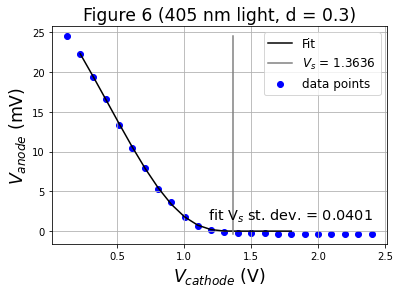
\includegraphics[scale=0.5]{fig6.png}
\end{center}
Here the stopping voltage for reduced-intensity light of $\lambda = 405\, nm$ is $1.3636\pm 0.0401\, V$. \newpage


Now we perform the fitting procedure for the full-intensity light data. For the incident light of wavelength $635\, nm$, the best fit values and the standard deviations of the parameters are given by the followings:
\begin{center}
\begin{tabular}{|c|c|c|c|c|}
\hline
 & a & b & c & $V_s$\\
\hline
best fit value & 569.1897 & -2151.0230 & -14.3998 & 0.3912\\
\hline
standard deviation & 43.8081 & 149.7486 & 2.4877 & 0.0065 \\
\hline
\end{tabular}\\
\hfill\break
\hfill\break
\hfill\break
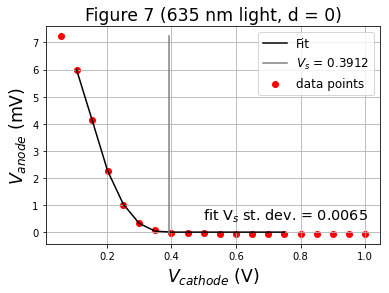
\includegraphics[scale=0.5]{fig7.png}
\end{center}
Here we see that the stopping voltage for full-intensity light of $\lambda = 635\, nm$ is estimated to be $0.3912\pm 0.0065\, V$, which falls within one standard deviation from the estimation of that of the reduced-intensity light of the same wavelength. \\

For the full-intensity light of wavelength $532\, nm$, the fitted parameters are given by: \begin{center}
\hfill\break
\begin{tabular}{|c|c|c|c|c|}
\hline
 & a & b & c & $V_s$\\
\hline
best fit value & 54.7024 & -24.8958 & 2.5582 & 0.6714\\
\hline
standard deviation & 15.2971 & 189.9723 & 12.172 & 0.0094 \\
\hline
\end{tabular}\\
\hfill\break
\hfill\break
\hfill\break
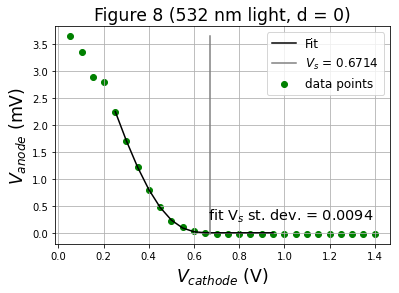
\includegraphics[scale=0.5]{fig8.png}
\end{center}
Here we see that the stopping voltage for full-intensity light of $\lambda = 532\, nm$ is estimated to be $0.6714\pm 0.0094\, V$, which also falls within one standard deviation from that of the half-intensity light of the same wavelength. \\

For the reduced-intensity light of wavelength $405\, nm$, the fitted parameters are given by:

\begin{center}
\begin{tabular}{|c|c|c|c|c|}
\hline
 & a & b & c & $V_s$\\
\hline
best fit value & 124.987 & -22.9975 & 1.4588 & 1.3394 \\
\hline
standard deviation & 35.9933 & 26.4706 & 1.2834 & 0.0379 \\
\hline
\end{tabular}\\
\hfill\break
\hfill\break
\hfill\break
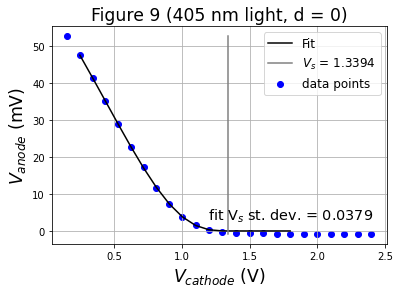
\includegraphics[scale=0.5]{fig9.png}
\end{center}
Here we see that the stopping voltage for full-intensity light of $\lambda = 405\, nm$ is estimated to be $1.3394\pm 0.0379\, V$, which also falls within one standard deviation from that of the half-intensity light of the same wavelength. \\

In all wavelengths, we see that the difference between the estimated stopping voltage with or without the density filter is small (less than one standard deviation), which leads to the conclusion that the stopping voltage is independent on the intensity of the incident light. While on the other hand, we see that the stopping voltage increases as wavelength of the incident light decreases. Since we have $f = 1/\lambda$, this confirms that stopping voltage increases as frequency of incident light increases. This result is well predicted by equation (3.2), and we will verify the linear relationship between the two in the next section. \\


\subsection{Determining the Planck's constant}
In this section, we fit out data using equation (3.2) to find the Planck's constant:
\begin{align*}
eV_s = hf - e\phi \tag{3.2}
\end{align*}
where $V_s$ is obtained from the last section. Here we have two parameters to fit, the Planck's constant $h$ and the work function $e\phi$ of the cathode material. We have two sets of data, the one without the density filter, and the one with the density filter. Again, we use the Python scipy function \textit{optimize.curve$\_$fit} to get the results. \\

We start by fitting the set with the density filter. The best-fit parameters that we obtain  and their standard deviation are given by the followings:
\begin{center}
\begin{tabular}{|c|c|c|}
\hline
 & $h$ & $\phi$ \\
\hline 
best fit value & $5.7191\cdot 10^{-34}$ & $1.3123$\\
\hline
standard deviation & $2.8751 \cdot 10^{-35}$ & $0.1081$\\
\hline
\end{tabular}
\end{center}
For the one without the density filter, the parameters are given by the followings:
\begin{center}
\begin{tabular}{|c|c|c|}
\hline
 & $h$ & $\phi$ \\
\hline 
best fit value & $5.8776\cdot 10^{-34}$ & $1.3613$\\
\hline
standard deviation & $2.8384 \cdot 10^{-35}$ & $0.1067$\\
\hline
\end{tabular}
\end{center}


\begin{center}
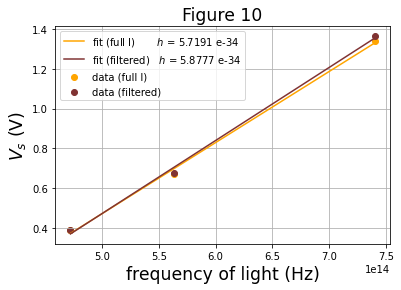
\includegraphics[scale=0.5]{fig10.png}
\end{center}

The theoretical value for $h$ is given by:
\begin{align*}
h = 6.6261 \cdot 10^{-34}\, m^2 \,kg /s
\end{align*}
which differs from each of the experimental values that we estimated using the two data sets by more than $3$ standard deviations:
\begin{align*}
\begin{cases}
h=(5.7197\pm 0.2875) \cdot 10^{-34} \, m^2 \,kg /s  & \text{reduced-intensity}\\
h=(5.8776\pm 0.2838) \cdot 10^{-34} \, m^2 \,kg /s  & \text{full-intensity}\\
\end{cases}
\end{align*}
hence we are not able to statistically verify the theoretical value of the Planck's constant. This result is most likely due to the stray light that impinges on the phototube anode and cathode. Even though efforts have been made, such as covering the box on the gray foam pad when taking data, to avoid the effect of stray light, it is experimentally difficult to completely block the stray light because the box is not airtight. To get a more precise measurement of the Planck's constant, one might need to design the experiment in another way to minimize the effect of the stray light. Nevertheless, the results from our data, as shown in Fig. 10, do justify a linear relationship between the frequency of the incident light and the stopping voltage $V_s$, and this result is well predicted by equation (3.2).\\

Lastly, according to Toshimichi Sakata, the work function for the Cs$_3$Sb photo-cathode material is around $(1.8\pm0.1)\, eV$.$^{[3]}$ In our experimental data, the work function of the photo-cathode is estimated to be:
\begin{align*}
\begin{cases}
(1.3123\pm 0.1081)\, eV & \text{reduced-intensity}\\
(1.3613 \pm 0.1067)\, eV& \text{full-intensity}
\end{cases}
\end{align*}
hence we see that the theoretical value of the work function differs from our experimental value by more than $3$ standard deviation, in which case we are not able to conclude that the experimental result agrees with the theoretical value. And again, this is most like due to the effect of stray light that impinges on the phototube anode and cathode.\\


\hfill\break
\hfill\break
\section{Summary}
In this lab, intending to verify the universal relationship in the photoelectric effect given by equation (3.1) and (3.2), we found that the stopping voltage of the photocurrent is independent of the intensity of the incident light by comparing our experimental data obtained with and without the density filter. Even though we were not able to verify the theoretical value of the Planck's constant and the work function of the cathode using our experimental data, our data does confirm that the relationship between the stopping voltage and the frequency of the incident light is linear as predicted by equation (3.2). \\
\hfill\break
\hfill\break

\section{References}
\begin{enumerate}
\item \textit{Über den Einfluss des ultravioletten Lichtes auf die electrische Entladung},  Heinrich  Hertz, Annalen der Physik 267, 983–1000 (1887). 
\item \textit{Über  einen  die  Erzeugung  und  Verwandlung  des  Lichtes  betreffenden  heuristischen Gesichtspunkt}, [\textit{On a Heuristic Viewpoint Concerning the Production and Transformation of Light}], Albert Einstein, Annalen der Physik 17, 132–148 (1905).
\item \textit{Studies on the Cs3Sb Photo-Cathode}, Toshimichi Sakata, Journal of the Physical Society of Japan 8, 723-730 (1953). 
\end{enumerate}


\newpage
\section{Experiment Data}
\begin{center}
\begin{tabular}{|c|c|c|}%
\hline
	\textbf{green (532 nm)} & &   \\
\hline	
     \bfseries Vcathode & \bfseries Vanode &\bfseries Vanode0.3 % specify table head
    \csvreader[head to column names]{green_data_532.csv}{}% use head of csv as column names
    {\\\hline\csvcoli&\csvcolii&\csvcoliii}\\% specify your coloumns here
\hline  
\end{tabular}  \\
\hfill\break
\hfill\break
\begin{tabular}{|c|c|c|}
\hline
	\textbf{red (635 nm)} & &   \\
\hline	
     \bfseries Vcathode & \bfseries Vanode &\bfseries Vanode0.3 % specify table head
    \csvreader[head to column names]{red_data_635.csv}{}% use head of csv as column names
    {\\\hline\csvcoli&\csvcolii&\csvcoliii}\\% specify your coloumns here
\hline    
\end{tabular}

\newpage
\begin{tabular}{|l|c|c|c|}
\hline
	\textbf{blue (405 nm)} & &   \\
\hline	
     \bfseries Vcathode & \bfseries Vanode &\bfseries Vanode0.3 % specify table head
    \csvreader[head to column names]{blue_data_405.csv}{}% use head of csv as column names
    {\\\hline\csvcoli&\csvcolii&\csvcoliii}\\% specify your coloumns here
\hline    
\end{tabular}
\end{center}
\newpage

\section{Code}
The code for computing statistics of the data sets is attached.
\lstset{style=mystyle}
\lstinputlisting[language=Python]{code.py}


\end{document}